\subsection{Neurális hálók}

\begin{frame}{Neurális hálók}
    \centering
    \begin{tikzpicture}
        \node<1> (img1) {\includegraphics[scale=0.34]{figures/neuron.png}};
        \node<2> (img2) {\includegraphics[scale=0.34]{figures/neuron-model.png}};
    \end{tikzpicture}
\end{frame}

\begin{frame}{Neurális hálók}
    Első matematikai leírás: McCulloch and Pitts (1943)
    
    \centering
    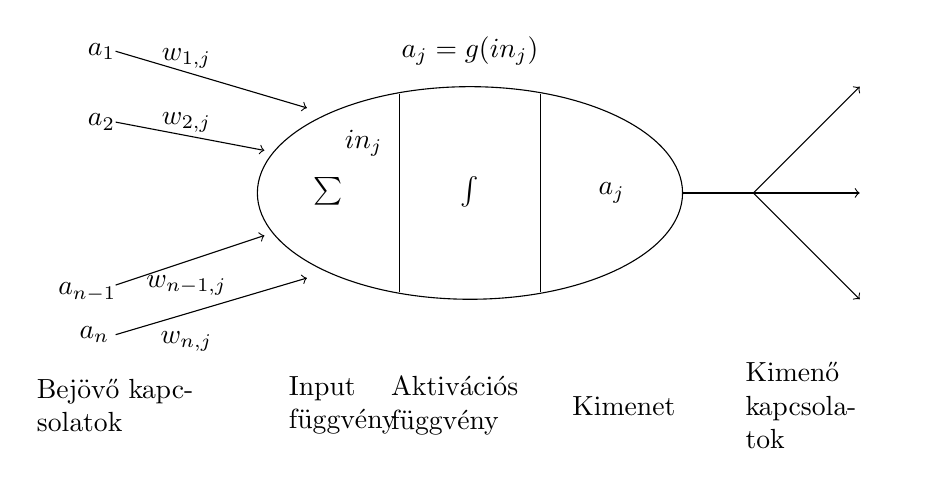
\begin{tikzpicture}[scale=0.9]
        \draw[->] (-5,2) -- (-2.3,1.2);
        \draw[->] (-5,1) -- (-2.9,0.6);
        \draw[->] (-5,-1.3) -- (-2.9,-0.6);
        \draw[->] (-5,-2) -- (-2.3,-1.2);
        \draw (-5.2,2) node{$a_1$};
        \draw (-5.2,1) node{$a_2$};
        \draw (-5.4,-1.4) node{$a_{n-1}$};
        \draw (-5.3,-2) node{$a_n$};
        \draw (-4,1.9) node{$w_{1,j}$};
        \draw (-4,1) node{$w_{2,j}$};
        \draw (-4,-1.3) node{$w_{n-1,j}$};
        \draw (-4,-2.1) node{$w_{n,j}$};
        
        \draw (0,0) ellipse [x radius=3cm, y radius=1.5cm];
        \draw (-2,0) node{\Huge{$\sum$}};
        \draw (-1.5,0.7) node{$in_j$};
        \draw (-1,1.4) -- (-1,-1.4);
        \draw (0,0) node{\Huge{$\int$}};
        \draw (1,1.4) -- (1,-1.4);
        \draw (2,0) node{$a_j$};
        \draw (0,2) node{$a_j=g(in_j)$};
        
        \draw (3,0) -- (4,0);
        \draw[->] (4,0) -- (5.5,1.5);
        \draw[->] (4,0) -- (5.5,0);
        \draw[->] (4,0) -- (5.5,-1.5);
        \draw (-5,-3) node[text width=2cm]{Bejövő kapcsolatok};
        \draw (-2,-3) node[text width=1cm]{Input függvény};
        \draw (0,-3) node[text width=2cm]{Aktivációs függvény};
        \draw (2,-3) node[text width=1cm]{Kimenet};
        \draw (5,-3) node[text width=2cm]{Kimenő kapcsolatok};
    \end{tikzpicture}
\end{frame}

\begin{frame}{Neurális hálók - aktivációs függvények}
    \hspace*{-1.5cm}
    \includegraphics[width=1.23\textwidth]{figures/activation_functions.pdf} \\
    ReLU = rectified linear units
\end{frame}

\begin{frame}{Neuráis hálók - Feed-forward háló}
    \centering
    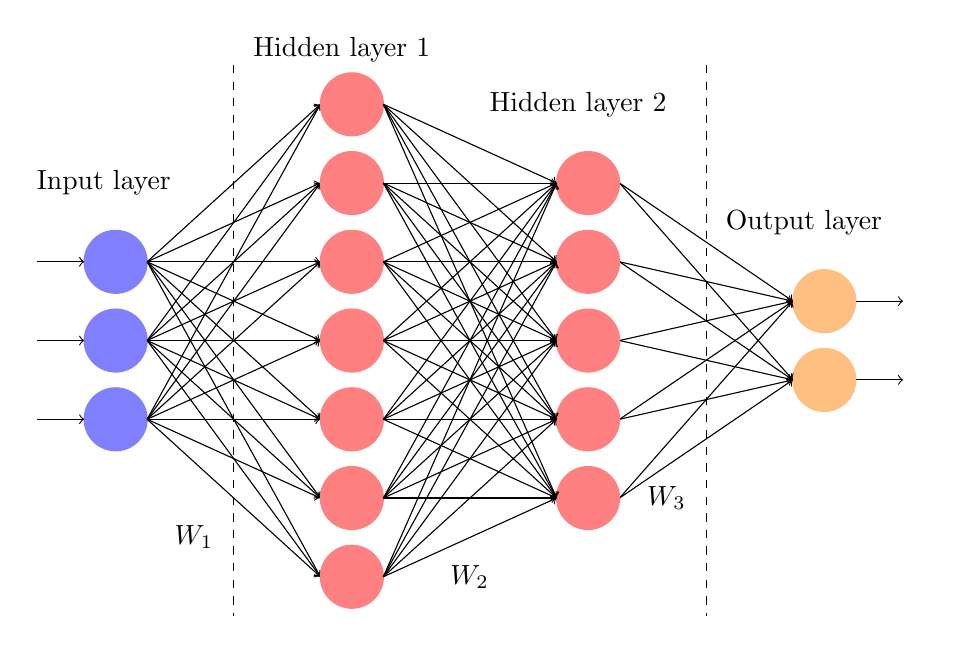
\begin{tikzpicture}
        % Input layer
        \foreach \y in {-1,0,1} {
            \draw[draw=blue!50,fill=blue!50] (-3, \y) circle [radius=0.4cm];  % Neuronok
            \draw[->] (-4, \y) -- (-3.4, \y);          % Inputba menő nyilak
            
            % Első hidden layer-be menő nyilak
            \foreach \yy in {-3,-2,-1,0,1,2,3} {
                \draw[->] (-2.6, \y) -- (-0.4, \yy);
            }
        }
        
        % Output layer
        \foreach \y in {0.5,-0.5} {
            \draw[draw=orange!50,fill=orange!50] (6,  \y) circle [radius=0.4cm];  % Neuronok
            \draw[->] (6.4, \y) -- (7, \y);            % Output-ból kimenő nyilak
            
            % Output layer-be menő nyilak
            \foreach \yy in {-2,-1,0,1,2} {
                \draw[->] (3.4, \yy) -- (5.6, \y);
            }
        }
        
        % Hidden layer 1
        \foreach \y in {-3,-2,-1,0,1,2,3} {
            \draw[draw=red!50,fill=red!50] (0, \y) circle [radius=0.4cm];
        }
        
        % Hidden layer 2
        \foreach \y in {-2,-1,0,1,2} {
            \draw[draw=red!50,fill=red!50] (3, \y) circle [radius=0.4cm];
        }
        
        % Hidden layer-ek közötti nyilak
        \foreach \y in {-3,-2,-1,0,1,2,3} {
            \foreach \yy in {-2,-1,0,1,2} {
                \draw[->] (0.4, \y) -- (2.6, \yy);
            }
        }
        
        % Feliratok
        \draw (-3,   2)   node[text width=2cm]   {Input layer};
        \draw ( 0,   3.7) node[text width=2.5cm] {Hidden layer 1};
        \draw ( 3,   3)   node[text width=2.5cm] {Hidden layer 2};
        \draw ( 6,   1.5) node[text width=2.5cm] {Output layer};
        \draw (-1,  -2.5) node[text width=2.5cm] {$W_1$};
        \draw ( 2.5,-3)   node[text width=2.5cm] {$W_2$};
        \draw ( 5.,-2)   node[text width=2.5cm] {$W_3$};
        
        % Elválasztó vonalak
        \draw[dashed] (-1.5, 3.5) -- (-1.5, -3.5);
        \draw[dashed] ( 4.5, 3.5) -- ( 4.5, -3.5);
    \end{tikzpicture}
\end{frame}


\begin{frame}{Neurális hálók}
    Problémák:
    \begin{itemize}
        \item Nincs általános háló
        \item Próbálgatással kell a jó hálót beállítani (vagy ügyesen megsejteni)
        \item Feed-forward hálók nem foglalkoznak a bemenet térbeli felépítésével
        \item Mennyi 
    \end{itemize}
    
    Megoldás: 
    \begin{itemize}
        \item Mély neurális hálók
        \item Konvolúciós neurális hálók
        \item Generatív modellek
    \end{itemize}
\end{frame}

